%! Author = matteomagnini
%! Date = 05/03/25

%----------------------------------------------------------------------------------------
\chapter{Autonomous learning systems}
\label{ch:autonomous-learning-systems}
\minitoc
%----------------------------------------------------------------------------------------


This is arguably the most important chapter of the thesis, the crucial moment when all the bricks come together.
%
In the following sections, we will present key contributions of the PhD towards the development of autonomous learning systems exploiting \gls{SKI} and \gls{SKE}.
%



\section{Goals and challenges}\label{sec:goals-and-challenges}
\note{Add references for this section}
%
The goal of autonomous learning systems is straightforward: to create systems that can learn -- and possibly adapt -- independently, without requiring constant human intervention.
%
The knowledge that is learnt can be presented in many forms.
%
We discussed in details about the differences between symbolic and sub-symbolic representations in ~\Cref{ch:ai} and also the many forms of symbolic knowledge that can be used to represent knowledge, such as rules, ontologies, and knowledge graphs~\Cref{sec:symbolic-ai}.
%
We believe that the knowledge learnt by autonomous learning systems should be represented symbolically.
%
The advantages of symbolic representations are many, as we discussed in~\Cref{sec:symbolic-ai}.
%
Here, we recall the most important ones:
%
\begin{inlinelist}
    \item interpretability: symbolic knowledge is human-readable, which makes it easier to understand and verify;
    \item reasoning: symbolic knowledge can be used to perform logical reasoning;
    \item transferability: symbolic knowledge can be easily transferred between different systems and domains, which makes it more versatile;
    \item model compression: symbolic knowledge can be more compact than sub-symbolic representations, which makes it more efficient;
    \item model checking: symbolic knowledge can be formally verified, which makes it more reliable.
\end{inlinelist}


On the other hand, sub-symbolic models have recently reached impressive performance in many tasks, especially in \gls{NLP} and \gls{NLG}, thanks to the advent of \glspl{LLM}.
%
Indeed, \glspl{LLM} are de-facto the new drivers of \gls{AI}.
%
Their presence is already ubiquitous, and they are used daily by millions of people.
%
Many \glspl{LLM} are so good at understanding and generating natural language that they can be considered as domain experts in many fields.
%
Still, limitations exist, and the possibility to generate hallucinations is always present.


In the following sections, we will present two main contributions of this PhD towards the development of autonomous learning systems.
%
Both contributions exploit \glspl{LLM} to generate or finetune symbolic knowledge about specific domains.



\section{\Glspl{LLM} as oracles for instantiating ontologies with domain-specific knowledge}
\label{sec:llm-as-oracles-for-instantiating-ontologies-with-domain-specific-knowledge}
%
The demand for intelligent systems capable of understanding, reasoning, and interacting with complex information is rapidly increasing.
%
The development of such systems relies on the integration of machine-interpretable knowledge representations that can encapsulate human domain-specific knowledge across diverse fields.


The proliferation of data and its varied representation formats raises the question: \emph{How can domain-specific information be precisely represented in a machine-understandable manner?}
%
The answer lies in the concept of ontology~\cite{placeholder}.
%
Ontologies are formal, extensional representations of knowledge based on the principles of \glspl{DL}.
%
They define concepts, relationships, and properties in a structured, machine-readable format, enabling computational systems to reason about the world in a manner akin to human cognition.


Unlike sub-symbolic approaches, which rely on distributed or loosely organized data~\cite{placeholder}, ontologies provide a structured framework.
%
This framework bridges the \emph{semantic gap}, allowing \gls{AI} systems to move beyond superficial pattern recognition and grasp the underlying meaning of data.
%
From a human perspective, ontologies offer a shared vocabulary and an unambiguous understanding of domain-specific knowledge.
%
However, creating ontologies is a meticulous and time-consuming process, requiring adherence to the real-world domain they represent.


Currently, ontology population is performed either manually by domain experts or communities, or through semi-automatic extraction from data~\cite{placeholder}.
%
Manual population, while time-intensive and prone to human error, can yield high-quality results if the process is thorough and inclusive.
%
In contrast, data-driven approaches offer speed and scalability but may result in lower-quality ontologies due to biases in the data or limitations in the extraction process.


An ideal ontology population method would combine human- and data-driven approaches.
%
The former would refine and validate the ontology, while the latter would provide the necessary volume of instances.
%
To this end, we introduce \llmfkg, a novel approach that amalgamates the strengths of both methods.


Leveraging the observation that \glspl{LLM} are trained on diverse data from the web, we hypothesize that these models encapsulate substantial domain-specific knowledge.
%
\llmfkg{} is an automated procedure designed to extract this knowledge from \glspl{LLM} and use it to populate ontologies.
%
Starting with an initial schema of interrelated classes and properties, and a set of query templates, the method queries the \gls{LLM} multiple times.
%
It generates instances for classes, relationships, and properties based on the responses.
%
Further queries refine the ontology and balance the class hierarchy, ensuring compliance with the initial schema.
%
The result is an enriched ontology that experts can review, adjust, or complement as needed.


Our method has several advantages over state-of-the-art approaches.
%
First, it is not tied to any specific dataset, as it uses \glspl{LLM} as oracles to generate data.
%
Second, it supports both ontology population and refinement, making it incremental and applicable to pre-existing ontologies.
%
Finally, it is general-purpose, suitable for various domains and different \glspl{LLM}.

%

To validate our approach, we implemented \llmfkg{} in Python and used it to populate a custom \gls{OWL} ontology.
%
We evaluated the quality of the populated ontology through a detailed inspection of the generated instances, assessing their meaningfulness and placement within the ontology structure.
%
The experiment was repeated with different \glspl{LLM}, and the results were compared.


In summary, our method contributes to the ongoing discourse on ontology population by presenting a hybrid approach that leverages the capabilities of \glspl{LLM}.
%
To further analyze the strengths, weaknesses, opportunities, and threats of our approach, we dedicate a section to a detailed \gls{SWOT} analysis.


\subsection{Related work}
\label{subsec:related-work-kgfiller}

\paragraph{Ontology Population}
\label{par:related-workd-ontology-population}
%
The task of populating ontologies with instances, commonly referred to as \emph{ontology population}, is well-established in the semantic web community~\cite{placeholder}.
%
This process involves expanding an ontology with additional assertions, also known as \emph{ABox axioms}, while ensuring compliance with the concepts and properties defined in the \emph{TBox axioms}.
%
Some authors use the term \emph{ontology learning} to emphasize the (semi-)automatic inference of the entire ontology, including TBox axioms~\cite{placeholder}.
%
However, in this work, we adhere to the term \emph{ontology population}.


The need for (semi-)automatic ontology population arises from the limitations of manual methods, which are time-consuming, error-prone, and inherently costly~\cite{placeholder}.
%
To address these challenges, various methods for structured data extraction from text have been proposed.
%
These methods can be broadly categorized into \emph{linguistics-based} and \gls{ML} approaches~\cite{placeholder}.


Linguistics-based approaches~\cite{placeholder} include techniques such as syntactic analysis, pattern-based extraction, part-of-speech tagging, and the use of dictionaries.
%
While effective, these methods require significant human effort for tasks like corpus selection, supervision, and parameter fine-tuning.
%
Additionally, they are often domain-specific, as different corpora may yield varying statistical information, necessitating tailored thresholds.


ML-based approaches can be further divided into \emph{shallow \gls{ML}} and \emph{deep learning} techniques.
%
Shallow ML methods rely on classical \gls{NLP} techniques, such as term frequency-inverse document frequency (TF-IDF), to convert text into numerical data, which is then processed by algorithms like decision trees~\cite{placeholder}.
%
However, these methods often struggle to capture contextual information.
%
In contrast, deep learning approaches automatically learn representations from data, enabling them to better capture contextual nuances~\cite{placeholder}.


Despite their advancements, all these methods require a large corpus of textual documents for extracting concepts, instances, and properties.
%
This reliance on external data introduces challenges such as bias, incompleteness, and domain non-representativeness.
%
Moreover, state-of-the-art methods are highly domain-sensitive and lack incrementality.
%
Domain sensitivity refers to the difficulty of finding sufficient relevant documents for narrow domains or avoiding irrelevant information in broad domains.
%
Poor incrementality implies that once an ontology is populated, adding new instances often requires re-populating it from scratch.


\paragraph{\glspl{LLM} and Knowledge Graphs}
\label{par:related-works-on-llm-and-knowledge-graphs}
%
In recent years, \glspl{LLM} have been applied to (semi-)automatic manipulation of \glspl{KG}~\cite{placeholder}.
%
\glspl{KG} represent knowledge as structured triplets of the form \((s, p, o)\), where \(s\) is the subject, \(p\) the predicate, and \(o\) the object.
%
Unlike ontologies, \glspl{KG} do not impose strict schema constraints, making them more flexible but less amenable to automated reasoning~\cite{placeholder}.
%
Conversely, ontologies use a well-defined set of axioms, ensuring compliance with the original schema.
%
Applications of \glspl{LLM} to \glspl{KG} can be categorized into \emph{\gls{KG} completion} and \emph{\gls{KG} construction}.


\Gls{KG} completion involves predicting missing facts, where \glspl{LLM} act as either \emph{encoders} or \emph{generators}.
%
As encoders, \glspl{LLM} encode textual information to assist another model in predicting missing facts~\cite{placeholder}.
%
As generators, they directly extract missing facts~\cite{placeholder}.
%
However, these methods often require input text or ad-hoc training, which our approach does not.


\Gls{KG} construction involves building a \gls{KG} from scratch, including tasks like entity discovery, end-to-end construction, and KG distillation.
%
Entity discovery identifies entities in text data and links them to form a \gls{KG}~\cite{placeholder}.
%
End-to-end methods generate \glspl{KG} directly but rely on domain-specific textual data~\cite{placeholder}.
%
\Gls{KG} distillation uses \glspl{LLM} as oracles to generate triplets~\cite{placeholder}.
%
Notable examples include \texttt{Comet}~\cite{placeholder} and \texttt{Harvest}~\cite{placeholder}, which generate triplets based on prompts.
%
While similar to our method, these approaches are not tailored for ontologies and may produce inconsistent \glspl{KG}.
%
Additionally, they often require prompt engineering or specific training phases, which our method avoids.


\subsection{Filling Ontologies with \llmfkg}
\label{subsec:filling-ontologies-kgfiller}

\begin{figure}
    \centering
    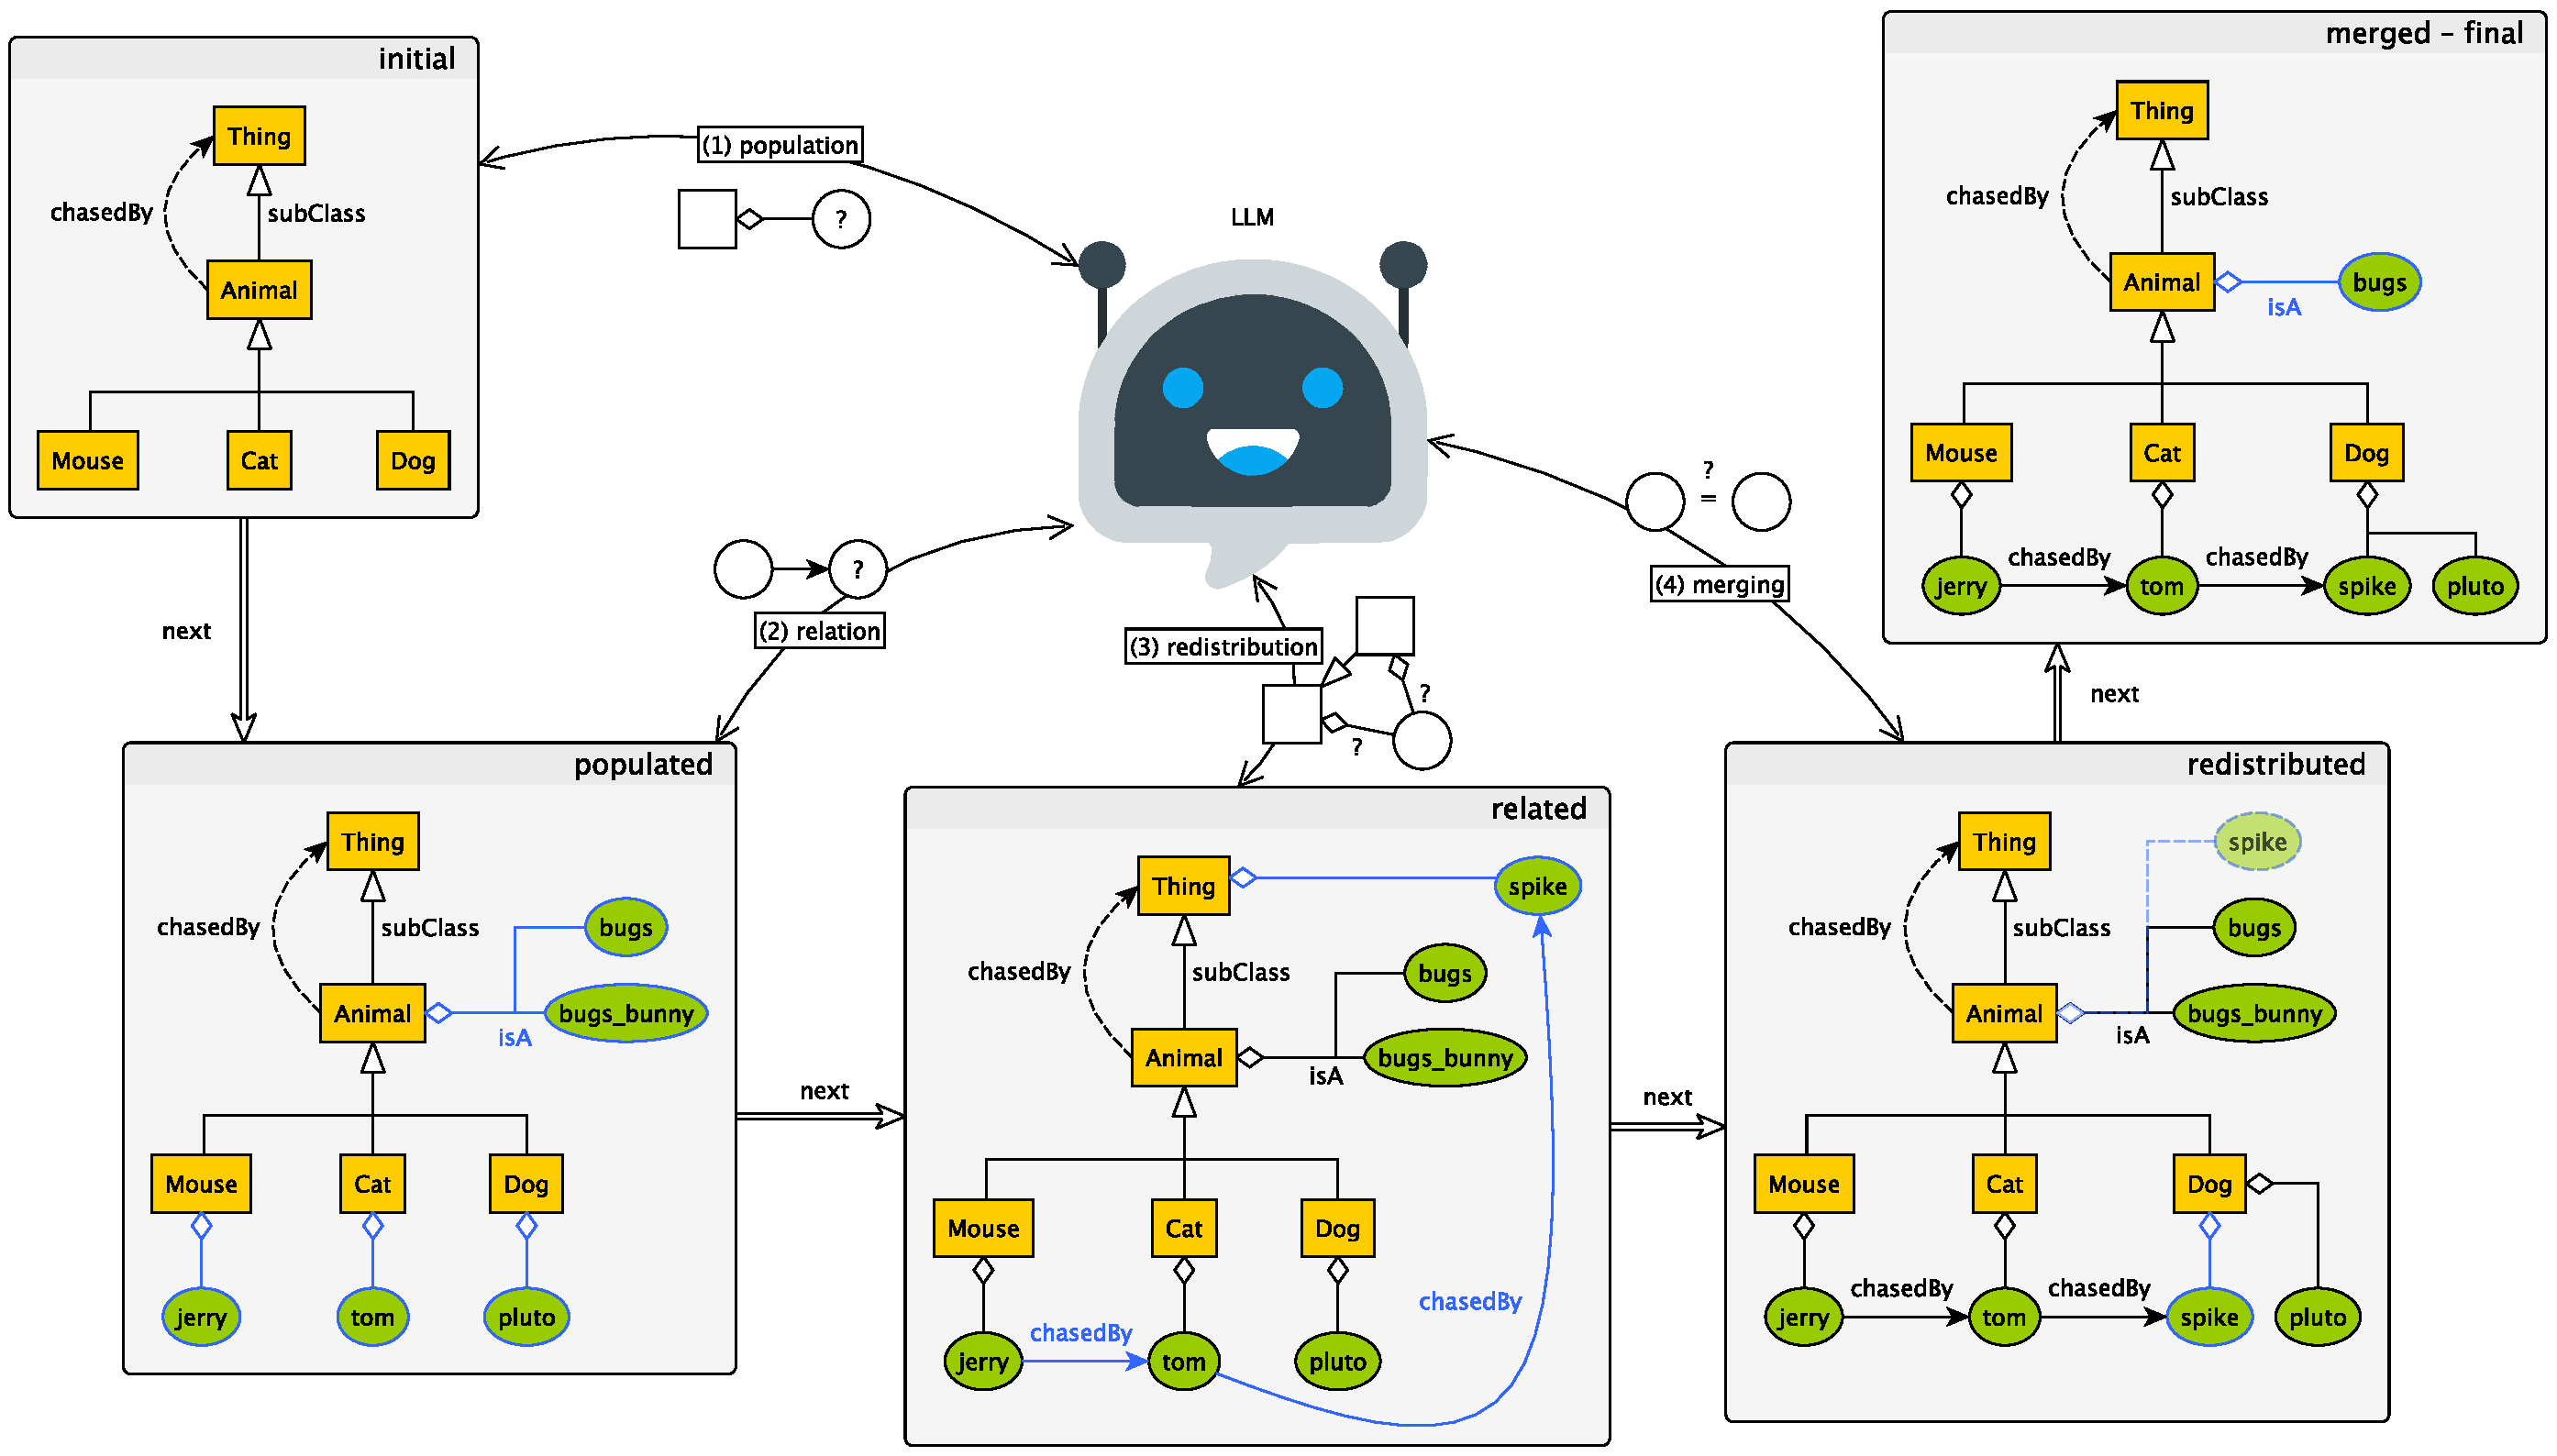
\includegraphics[width=\linewidth]{figures/kgfiller/roadmap}
    \caption{
        Overview of \llmfkg{}, illustrated with a running example.
        %
        The example assumes an ontology about animals, including classes such as $\concept{Cat}$, $\concept{Dog}$, and $\concept{Mouse}$, which are subclasses of $\concept{Animal}$, itself a subclass of $\concept{Thing}$ (\(\top\)).
        %
        Initially, the ontology contains no instances.
        %
        A property $\relation{chasedBy} : \concept{Animal} \times \top$ is defined, indicating that animals can be chased by other entities.
        %
        The figure outlines the four phases of the \llmfkg{} algorithm, with changes highlighted in blue.
    }
    \label{fig:roadmap}
\end{figure}

The \llmfkg{} framework is designed for semi-automatic ontology population, leveraging \glspl{LLM} as oracles.
%
This section provides a concise yet general description of the framework, with technical details discussed in Appendix~A.2.

%
\paragraph{Core Functionality}
\label{par:core-functionality}

At its core, \llmfkg{} operates on a partially instantiated ontology.
%
The ontology must include class and property definitions, organized hierarchically as a directed acyclic graph (DAG).
%
Classes may or may not have instances.

%
Class names should be meaningful, concise, and unambiguous to avoid issues during query generation for the \gls{LLM}.
%
The same applies to property names.

%
Given these assumptions, \llmfkg{} generates individuals for all classes and associates them using the ontology's properties.
%
Generated individuals are assigned meaningful names and placed in the most specific class available.

%
The framework supports two primary use cases:
%
\begin{inlinelist}
    \item ontology designers have defined the ontology's structure but lack instances, and
    %
    \item designers want to add more instances to an already populated ontology.
\end{inlinelist}
%
These use cases can be combined, allowing iterative rounds of population and manual refinement.

%
\paragraph{Query Templates}
\label{par:query-templates}

\llmfkg{} relies on query templates to generate questions for the \gls{LLM}.
%
Templates are text strings containing placeholders, which are replaced with actual values during execution.
%
For example, the template \(t = \text{``What is the capital of \(\langle c \rangle\)?''}\) can be instantiated with the substitution \(\sigma = \{\langle c \rangle \mapsto \text{``Italy''}\}\), resulting in \(t / \sigma = \text{``What is the capital of Italy?''}\).

%
We define four types of query templates:
%
\begin{itemize}
    \item \textbf{Individual-seeking templates:} Ask for instances of a class, e.g., ``Examples of \(\langle \text{class} \rangle\)?''.
    %
    \item \textbf{Relation-seeking templates:} Ask for individuals related to a given individual via a property, e.g., ``Examples of \(\langle \text{property} \rangle\) for \(\langle \text{individual} \rangle\)?''.
    %
    \item \textbf{Best-match templates:} Ask for the best class for an individual among candidates, e.g., ``What class is best for \(\langle \text{individual} \rangle\) among \(\langle \text{classes} \rangle\)?''.
    %
    \item \textbf{Individuals-merging templates:} Ask if two instances in a class are identical, e.g., ``In \(\langle \text{class} \rangle\), are \(\langle \text{ind1} \rangle\) and \(\langle \text{ind2} \rangle\) the same?''.
\end{itemize}

%
\paragraph{\gls{LLM} Oracle}
We do not impose constraints on the nature of the \gls{LLM} oracle or the underlying model.
%
\texttt{KGFiller} is agnostic to the specific \gls{LLM} used, as long as it supports generating textual responses from textual prompts.
%
Both prompts and responses are assumed to be strings of arbitrary length, written in a natural language.
%
The natural language must match the one used for naming classes and properties in the ontology.
%
Without loss of generality, we assume this language is English.
%
A key assumption is that the \gls{LLM} oracle is pre-trained on a large corpus of textual data, which includes domain-specific knowledge relevant to the ontology.


\paragraph{Problem Statement}
We formalize the ontology population problem addressed by \texttt{KGFiller} as follows:
%
\begin{enumerate}
    \item A partially instantiated ontology \(\mathcal{O} = \mathcal{C} \cup \mathcal{P} \cup \mathcal{I}\), where:
    %
    \begin{itemize}
        \item \(\mathcal{C} \neq \emptyset\) is a non-empty set of class definitions,
        \item \(\mathcal{P} \neq \emptyset\) is a non-empty set of property definitions, and
        \item \(\mathcal{I}\) is a possibly empty set of individuals and their relationships.
    \end{itemize}
    %
    \item A subsumption relation \(\sqsubseteq\) among the classes in \(\mathcal{C}\).
    %
    \item A set of query templates \(\mathcal{T} = \mathcal{T}_I \cup \mathcal{T}_R \cup \mathcal{T}_B \cup \mathcal{T}_M\), where:
    %
    \begin{itemize}
        \item \(\mathcal{T}_I\) contains individual-seeking templates,
        \item \(\mathcal{T}_R\) contains relation-seeking templates,
        \item \(\mathcal{T}_B\) contains best-match templates, and
        \item \(\mathcal{T}_M\) contains individuals-merging templates.
    \end{itemize}
    %
    \item A trained \gls{LLM} oracle \(\mathcal{L}\), encapsulating domain-specific knowledge.
\end{enumerate}

%

The goal of \texttt{KGFiller} is to generate a set of individuals and relationships \(\mathcal{I}'\) such that \(\mathcal{I} \subseteq \mathcal{I}'\).
%
All new individuals and relationships in \(\mathcal{I}'\) must be consistent with the class and property definitions in \(\mathcal{C}\) and \(\mathcal{P}\), respectively.
%
Specifically:
%
\begin{itemize}
    \item Every individual is associated with the most specific concept in \(\mathcal{C}\) with respect to \(\sqsubseteq\).
    %
    \item For every property in \(\mathcal{P}\), every individual in the property’s domain is associated with one or more individuals in the property’s range.
\end{itemize}


\paragraph{Phases}
To compute \(\mathcal{I}'\), \texttt{KGFiller} executes four sequential phases:
%
\begin{enumerate}
    \item \textbf{Population Phase:} Novel individuals are identified for each class in \(\mathcal{C}\).
    %
    \item \textbf{Relation Phase:} New relationships are identified for each property in \(\mathcal{P}\).
    %
    \item \textbf{Redistribution Phase:} Individuals are redistributed among the classes in \(\mathcal{C}\) to ensure each individual is placed in the most specific class available.
    %
    \item \textbf{Merge Phase:} Semantic duplicates within each class in \(\mathcal{C}\) are detected and merged.
\end{enumerate}
%
The order of these phases is critical.
%
The population phase generates individuals used in the relation phase, which may, in turn, generate additional individuals.
%
The redistribution phase ensures all individuals are placed in the most specific class, while the merge phase reduces semantic duplication.


\paragraph{Ancillary functions}
%
The next section introduces several auxiliary functions used throughout the framework.
%
The function \texttt{GetRange} (resp. \texttt{GetDomain}) retrieves the range (resp. domain) of a given property.
%
The function \texttt{AskOracle} models queries to the \gls{LLM} oracle, accepting and returning arbitrary strings.
%
The function \texttt{ExtractBinary} (resp. \texttt{ExtractNames}) extracts binary values (resp. relevant names of individuals or concepts) from the textual responses of the \gls{LLM}.
%
It returns a Boolean value (resp. a list of names) and accepts a string as input.
%
Finally, the function \texttt{AddToClass} assigns an individual to a class.
%
If the individual is already part of the class or any of its subclasses, the function performs no action.


\subsubsection{Population Phase}
\label{subsubsec:population-phase}
%
\begin{algorithm}
    \captionsetup{font=\algCaptionSize}
    \caption{Populates the given ontology with novel individuals queried from an LLM oracle}
    \label{alg:populate}
    \begin{algorithmic}[1]\algCodeSize
        \Require $\relset{O} = \relset{C} \cup \relset{P} \cup \relset{X}$: partially populated ontology
        \Require $\relset{T}_{I}$: individual seeking query templates
        \Require $\relset{L}$: LLM oracle
        \Require $\concept{R} \in \relset{C}$: root concept to be populated
        \Ensure $\relset{X}'$ contains novel individuals, assigned to the classes in $\relset{C}$
        \medskip
        \Function{\populate}{$\relset{O}, \relset{T}_I, \relset{L}, \concept{R}$}
            \State $\relset{X}' \gets \relset{X}$
            \ForAll{$\concept{C} \in \relset{C} \suchThat \concept{C} \sqsubset \concept{R} \wedge \concept{C} \neq \bot$}
                \State $\relset{O}' \gets \relset{C} \cup \relset{P} \cup \relset{X}'$
                \State $\relset{X}' \gets \Call{\populate}{\relset{O}', \relset{T}_{I}, \relset{L}, \concept{C}}$
            \EndFor
            \ForAll{$\mathit{t} \in \relset{T}_{I}$}
                \State $\mathit{q} \gets \mathit{t}/\{ \var{class} \mapsto \concept{R} \}$
                \State $\mathit{text} \gets \Call{\askOracle}{\relset{L}, \mathit{q}}$
                \ForAll{$\instance{i} \in \Call{\extractNames}{\mathit{text}}$}
                    \State $\relset{O}' \gets \relset{C} \cup \relset{P} \cup \relset{X}'$
                    \State $\relset{X}' \gets \Call{\addToClass}{\relset{O}', \instance{i}, \concept{R}}$
                \EndFor
            \EndFor
            \State \Return $\relset{X}'$
        \EndFunction
    \end{algorithmic}
\end{algorithm}
%
The population phase is based on the \populate{} function, as defined in \Cref{alg:populate}.
%
This function is designed to populate a partially instantiated ontology, denoted as $\relset{O}$, with new instances.
%
It achieves this by querying a \gls{LLM} oracle, represented as $\relset{L}$, using a set of instance-seeking query templates, $\relset{T}_{I}$.


The process begins with a root class $\concept{R} \in \relset{O}$.
%
The function then traverses the class hierarchy defined by the subsumption relation $\sqsubseteq$, following a depth-first post-order strategy.
%
This means that all direct and indirect subclasses of $\concept{R}$ are visited before $\concept{R}$ itself, ensuring that the most specific classes are populated first.
%
Such a strategy is crucial to guarantee that any individual generated during this phase is assigned to the most specific class available.


For each subclass $\concept{C} \sqsubseteq \concept{R}$, the function generates queries by replacing the placeholder $\var{class}$ in each template from $\relset{T}_{I}$ with the name of $\concept{C}$.
%
These queries are then submitted to the \gls{LLM} oracle $\relset{L}$, and the responses are processed to extract the names of the individuals.
%
The number of individuals generated per query is unbounded and depends on the capabilities of the \gls{LLM} oracle $\relset{L}$ and other implementation-specific factors~\cite{placeholder}.


It is possible for the same individual to be generated by multiple queries or for multiple subclasses of $\concept{R}$.
%
However, this does not pose any issues, as the \addToClass{} function ensures that individuals are not duplicated and are always assigned to the most specific class.
%
This behavior aligns with the post-order exploration strategy, which prioritizes the population of specific concepts over more general ones.


To populate the entire ontology $\relset{O}$, the function can be invoked with the top class $\top$ as the root:
%
\Call{\populate}{$\relset{O}, \relset{T}_I, \relset{L}, \top$}.
%
This ensures that all classes in $\relset{O}$ are visited and populated systematically.


\subsubsection{Relation Phase}
\label{subsubsec:relation-phase}
%
\begin{algorithm}
    \captionsetup{font=\algCaptionSize}
    \caption{Populates the given ontology with novel relationships queried from an LLM oracle}
    \label{alg:relate}
    \begin{algorithmic}[1]\algCodeSize
        \Require $\relset{O} = \relset{C} \cup \relset{P} \cup \relset{X}$: partially populated ontology
        \Require $\relset{T}_{R}$: relation seeking query templates
        \Require $\relset{L}$: LLM oracle
        \Require $\relation{P} \in \relset{P}$: property to be populated
        \Ensure $\relset{X}'$ contains novel relationships, involving individuals in $\relset{X}$
        \medskip
        \Function{\relate}{$\relset{O}, \relset{T}_R, \relset{L}, \relation{P}$}
            \State $\relset{X}' \gets \relset{X}$
            \State $\concept{D} \gets \Call{\getDomain}{\relation{P}}$
            \State $\concept{R} \gets \Call{\getRange}{\relation{P}}$
            \ForAll{$(\instance{i} : \concept{D}) \in \relset{X}$}
                \ForAll{$\mathit{t} \in \relset{T}_{R}$}
                    \State $\mathit{q} \gets \mathit{t}/\{ \var{individual} \!\mapsto\! \instance{i}, \var{property} \!\mapsto\! \relation{P} \}$
                    \State $\mathit{text} \gets \Call{\askOracle}{\relset{L}, \mathit{q}}$
                    \ForAll{$\instance{i}' \in \Call{\extractNames}{\mathit{text}}$}
                        \State $\relset{O}' \gets \relset{C} \cup \relset{P} \cup \relset{X}'$
                        \State $\relset{X}' \gets \Call{\addToClass}{\relset{O}', \instance{i}', \concept{R}}$
                        \State $\relset{X}' \gets \relset{X}' \cup \{ \relation{P}(\instance{i}, \instance{i}') \}$
                    \EndFor
                \EndFor
            \EndFor
            \State \Return $\relset{X}'$
        \EndFunction
    \end{algorithmic}
\end{algorithm}
%
The relation phase utilizes the \relate{} function to populate a partially instantiated ontology, \(\relset{O}\), with new relationships.
%
These relationships link existing individuals and may introduce novel individuals, based on queries to a \gls{LLM} oracle, \(\relset{L}\), using a set of relation-seeking query templates, \(\relset{T}_{R}\).

%
Consider a property \(\relation{p} \in \relset{O}\), defined as \(\relation{p} : \concept{D} \times \concept{R}\), where \(\concept{D}\) and \(\concept{R}\) represent the domain and range of \(\relation{p}\), respectively.
%
The function queries the \gls{LLM} oracle, \(\relset{L}\), to identify relationships between each individual \(\instance{i} \in \concept{D}\) and potential individuals \(\instance{i}' \in \concept{R}\) through \(\relation{p}\).

%
For each individual \(\instance{i}\) and each query template \(t \in \relset{T}_{R}\), a query \(q\) is generated by substituting placeholders \(\var{property}\) and \(\var{individual}\) in \(t\) with the names of \(\relation{p}\) and \(\instance{i}\), respectively.
%
The query \(q\) is submitted to the \gls{LLM} oracle, and the response is processed to extract the names of individuals to be added to the ontology.
%
Each new individual \(\instance{i}'\) is added to the range \(\concept{R}\) of \(\relation{p}\), along with the relationship \(\relation{p}(\instance{i}, \instance{i}')\).

%
To populate relationships for all properties \(\relation{p} \in \relset{O}\), the function is invoked for each property as follows:
%
\Call{\relate}{$\relset{O}, \relset{T}_R, \relset{L}, \relation{p}$}.

%
It is important to note that the \relate{} function may generate new individuals during its execution.
%
In some cases, the range \(\concept{R}\) of the property \(\relation{p}\) may not be the most specific class for these individuals.
%
For example, a subclass \(\concept{C} \sqsubset \concept{R}\) might better represent some of the generated individuals.
%
This necessitates the redistribution phase, which ensures that all individuals are assigned to the most specific class available.


\subsubsection{Redistribution Phase}
\label{subsubsec:redistribution-phase}
%
\begin{algorithm}
    \captionsetup{font=\algCaptionSize}
    \caption{Redistributes individuals from the given ontology's classes, in such a way that each individual is assigned to the most specific class available}
    \label{alg:redistribute}
    \begin{algorithmic}[1]\algCodeSize
        \Require $\relset{O} = \relset{C} \cup \relset{P} \cup \relset{X}$: partially populated ontology
        \Require $\relset{T}_{B}$: relation seeking query templates
        \Require $\relset{L}$: LLM oracle
        \Require $\concept{R} \in \relset{C}$: root concept within which redistribution should occur
        \Ensure $\relset{X}'$ contains the different assignments of individuals to classes
        \medskip
        \Function{\redistribute}{$\relset{O}, \relset{T}_B, \relset{L}, \concept{R}$}
            \State $\relset{X}' \gets \relset{X}$
            \State $\relset{S} \gets \{ \concept{S} \in \relset{C} \mid \concept{S} \sqsubset \concept{R} \}$
            \ForAll{$(\instance{i} : \concept{R}) \in \relset{X}'$}
                \State $\concept{B} \gets \concept{R}$
                \ForAll{$\mathit{t} \in \relset{T}_{B}$}
                    \State $\mathit{q} \gets \mathit{t}/\{ \var{individual} \mapsto \instance{i}, \var{classes} \mapsto \relset{S} \}$
                    \State $\mathit{text} \gets \Call{\askOracle}{\relset{L}, \mathit{q}}$
                    \ForAll{$\concept{C} \in \Call{\extractNames}{\mathit{text}}$}
                        \State $\concept{B} \gets \concept{C}$
                        \State \Break{going to line \ref{line:first-result}}
                    \EndFor
                \EndFor
                \State $\relset{O}' \gets \relset{C} \cup \relset{P} \cup \relset{X}'$ \label{line:first-result}
                \State $\relset{X}' \gets \Call{\addToClass}{\relset{O}', \instance{i}, \concept{B}}$
            \EndFor
            \ForAll{$\concept{C} \in \relset{C} \suchThat \concept{C} \sqsubset \concept{R} \wedge \concept{C} \neq \bot$}
                \State $\relset{O}' \gets \relset{C} \cup \relset{P} \cup \relset{X}'$
                \State $\relset{X}' \gets \Call{\redistribute}{\relset{O}', \relset{T}_{B}, \relset{L}, \concept{C}}$
            \EndFor
            \State \Return $\relset{X}'$
        \EndFunction
    \end{algorithmic}
\end{algorithm}
%
The redistribution phase utilizes the \redistribute{} function, as defined in \Cref{alg:redistribute}.
%
This function redistributes individuals among the classes of an instantiated ontology, \(\relset{O}\), ensuring that each individual is assigned to the most specific class available.
%
To achieve this, the function queries the \gls{LLM} oracle, \(\relset{L}\), using a set of best-match query templates, \(\relset{T}_{B}\).

%
Starting from a root class \(\concept{R} \in \relset{O}\), the function recursively explores the class hierarchy defined by the subsumption relation \(\sqsubseteq\).
%
It follows a depth-first pre-order traversal strategy, visiting each class before its subclasses.
%
This approach ensures that individuals can be reassigned to more specific classes as the traversal progresses.

%
For each visited class \(\concept{C} \sqsubseteq \concept{R}\), the function evaluates whether \(\concept{C}\) is the most appropriate class for all individuals currently assigned to it.
%
If a more specific subclass of \(\concept{C}\) is better suited for an individual, the function reassigns the individual accordingly.
%
For example, if \(\concept{Cat} \sqsubset \concept{Animal}\) and an individual \(\instance{tom}\) is initially assigned to \(\concept{Animal}\), the function reassigns \(\instance{tom}\) to \(\concept{Cat}\).

%
To determine the best class for an individual \(\instance{i} : \concept{C}\), the function generates a query for each template \(t \in \relset{T}_{B}\).
%
The placeholders \(\var{individual}\) and \(\var{classes}\) in \(t\) are replaced with the name of \(\instance{i}\) and the concatenated names of all direct subclasses of \(\concept{C}\), respectively.
%
The resulting query is submitted to the \gls{LLM} oracle, and the response is processed to extract candidate class names.
%
The first class in the response is selected as the best match, and \(\instance{i}\) is reassigned to it.

%
Since the function is recursive, an individual may be reassigned multiple times until it reaches the most specific class available in the ontology.
%
The depth-first pre-order strategy is crucial for this process, as it allows individuals to ``move down'' the class hierarchy efficiently while keeping query sizes manageable.

%
To redistribute all individuals in an ontology, the function can be invoked with the top class \(\top\) as the root:
%
\Call{\redistribute}{$\relset{O}, \relset{T}_{B}, \relset{L}, \top$}.
%
This ensures that every individual in \(\relset{O}\) is assessed and reassigned to the most specific class, if necessary.


\subsubsection{Merge Phase}
\label{subsubsec:merge-phase}
%
\begin{algorithm}
    \captionsetup{font=\algCaptionSize}
    \caption{Merges syntactically and semantically similar individuals from the given ontology's classes}
    \label{alg:merge}
    \begin{algorithmic}[1]\algCodeSize
        \Require $\relset{O} = \relset{C} \cup \relset{P} \cup \relset{X}$: partially populated ontology
        \Require $\relset{T}_{M}$: indivuals merging query templates
        \Require $\relset{L}$: LLM oracle
        \Require $\concept{R} \in \relset{C}$: root concept within which merge should occur
        \Ensure $\relset{X}'$ contains no duplicated individuals
        \medskip
        \Function{\merge}{$\relset{O}, \relset{T}_{M}, \relset{L}, \concept{R}$}
            \State $\relset{X}' \gets \relset{X}$
            \ForAll{$\concept{C} \in \relset{C} \suchThat \concept{C} \sqsubset \concept{R}$}
                \State $\mathcal{D} \gets \emptyset$
                \ForAll{$\instance{i}, \instance{j} : \concept{C} \suchThat ( \instance{i}, \instance{j} ) \in \relset{X}' \times \relset{X}'$}
                    \If{$\Call{\synSimilar}{\instance{i}, \instance{j}}$}
                        \State $\mathcal{D} \gets \mathcal{D} \cup \{\{\instance{i}, \instance{j}\}\}$
                    \EndIf
                \EndFor
                \ForAll{$\{ \instance{i}, \instance{j} \} \in \mathcal{D}$}
                    \ForAll{$\mathit{t} \in \relset{T}_{M}$}
                    \label{line:next-couple}
                        \State $\mathit{q} \gets \mathit{t}/\{ \var{ind_1}\!\mapsto\!\instance{i}, \var{ind_2}\!\mapsto\!\instance{j},
                            \var{class}\!\mapsto\!\concept{C} \}$
                        \State $\mathit{text} \gets \Call{\askOracle}{\relset{L}, \mathit{q}}$
                        \If{$\Call{\extractBinary}{text}$}
                            \State $\relset{X}' \gets \Call{\mergeInst}{i, j}$
                            \State \Break{going to line \ref{line:next-couple}}
                        \EndIf
                    \EndFor
                \EndFor
            \EndFor
        \EndFunction
    \end{algorithmic}
\end{algorithm}

%
The \merge{} function is responsible for identifying and merging duplicated individuals in an instantiated ontology, denoted as $\relset{O}$.
%
Duplicated individuals are defined as those with slightly different names but representing the same semantic entity.
%
Such duplicates often arise as a by-product of earlier phases in the ontology population process.


For example, consider the individuals $\instance{maincoone\_cat}$ and $\instance{maincoone}$, both belonging to the class $\concept{Cat} \sqsubset \concept{Animal}$.
%
Although their names differ syntactically, they refer to the same entity.
%
To address this, the \merge{} function queries the \gls{LLM} oracle, denoted as $\relset{L}$, to identify semantically similar individuals and merge them into a single entity.


The \merge{} function operates by scanning the ontology $\relset{O}$ for pairs of syntactically similar individuals.
%
For each pair, it uses a set of merging query templates, $\relset{T}_{M}$, to query the \gls{LLM} oracle.
%
The oracle's response determines whether the individuals should be merged.


The process begins with a root class $\concept{R} \in \relset{O}$ and recursively explores the class hierarchy defined by the subsumption relation $\sqsubseteq$.
%
For each class $\concept{C} \sqsubseteq \concept{R}$, the function identifies a set $\mathcal{D}$ of candidate duplicate pairs using the \synSimilar{} function.
%
Each pair is then evaluated using the \extractBinary{} function, which interprets the oracle's response as a Boolean value.
%
If the response is positive, the \mergeInst{} function is invoked to merge the individuals.
%
This involves transferring all information from one individual to the other and removing the redundant individual, resulting in an updated ontology $\relset{X}'$.


The merging process relies on templates in $\relset{T}_{M}$.
%
For each candidate pair, a query is generated by replacing the placeholders $\var{ind\_1}$, $\var{ind\_2}$, and $\var{class}$ in the template with the names of the individuals and the class $\concept{C}$, respectively.
%
The first template yielding a positive response is considered definitive, and further templates are not queried.
%
To ensure deterministic behavior and avoid issues arising from the oracle's creativity, the temperature parameter is set to 0.0 during these queries.


To detect and merge all duplicated individuals in an ontology $\relset{O}$, the function can be invoked as follows:
%
\Call{\merge}{$\relset{O}, \relset{T}_M, \relset{L}, \top$}.
%
This ensures that all classes in $\relset{O}$ are systematically visited, and any semantic duplicates are resolved.


\paragraph{Remarks}
%
\Cref{alg:merge} employs a post-order exploration strategy.
%
However, the choice of exploration strategy is \emph{not} critical for the merging phase.
%
Alternative strategies can be used, provided they visit all direct and indirect subclasses of $\concept{R}$.

%
The \synSimilar{} function plays a crucial role in determining whether two instances, $\instance{i}$ and $\instance{j}$, are sufficiently similar to be considered for merging.
%
Its implementation significantly impacts the overall performance of the \merge{} function~\cite{placeholder}.
%
% For example, one could define similarity based on shared substrings longer than a threshold $\lambda$.
% %
% Empirically, $\lambda$ can be set to 4 characters.

%
Regarding the merging phase, one might question why entity alignment approaches~\cite{ZhaoTkde2022} are not used.
%
While effective for identifying similar instances across different \glspl{KG}, these methods typically require additional domain-specific data~\cite{ChenIjcai2018,XuAcl2019}.
%
This is because entity alignment systems rely on ad-hoc \gls{ML} models trained for the alignment task, introducing extra complexity.

%
In contrast, our approach leverages the same \gls{LLM} oracle for both ontology population and duplicate identification.
%
Although not entirely error-free, this method avoids additional computational overhead during the population phase.
%
It also eliminates the need for users to provide extra domain-specific data or train additional models, simplifying the overall process.
%



\subsection{Case Study and Experiments}
\label{subsec:case-study}

This section presents a case study designed to empirically validate \llmfkg{}.

%
\subsubsection{Experimental Setup}
\label{subsubsec:experimental-setup}
%
The experimental setup involves designing a non-trivial ontology, as detailed in \Cref{ssec:ontology}.
%
The ontology includes a class hierarchy and a set of properties, which are populated using \llmfkg{}.
%
We fine-tune specific query templates (\Cref{ssec:query-templates}) and utilize various \glspl{LLM} from different families and technologies (\Cref{ssec:llms-oracles}).
%
This process generates a set of populated ontologies, all sharing the same structure but differing in their content.
%
The populated ontologies are analyzed and compared to evaluate the performance of \llmfkg{} and the impact of the chosen \gls{LLM} on the quality of the population process.
%
To achieve this, we define a taxonomy of errors and a set of metrics (\Cref{ssec:performance-metrics}) to measure the quality of the generated ontologies.
%
The evaluation is performed through a manual inspection of the populated ontologies, examining each individual and relationship (\Cref{ssec:results}).

%
Testing \llmfkg{} on a custom ontology, rather than a publicly available one, offers several advantages.
%
First, it allows precise control over the experiment's complexity and content.
%
Second, it avoids potential biases where \glspl{LLM} perform well due to prior exposure to the ontology during training.
%
However, this approach lacks ground truth data, making automatic validation infeasible.
%
Thus, manual inspection is necessary to identify errors and ensure the correctness of the algorithm's output.

%
\subsubsection{Code and Data}
\label{subsubsec:code-and-data}
%
The experiments are conducted using a Python implementation of \llmfkg{}, which is publicly available on GitHub\footnote{\url{https://github.com/Chistera4-Expectation/kg-filler}}.
%
The experimental results are also available on a dedicated repository\footnote{\url{https://github.com/Chistera4-Expectation/knowledge-graphs/branches}}, where each Git branch corresponds to a specific experiment.
%
The \texttt{main} branch contains the initial ontology, which includes only class and property definitions without any individuals.

%
For reproducibility, each experiment branch includes the populated ontology and the cache of query--response pairs from the \gls{LLM}.
%
This allows others to inspect the exact queries and responses and reproduce the experiments deterministically.
%
Additionally, the experiments are automated, with each commit in the branch corresponding to a single operation performed by \llmfkg{} (e.g., populating a class or property).
%
This commit history provides a detailed sequence of operations for each experiment.

%
\subsubsection{Ontology}
\label{subsubsec:kgfiller-ontology}
%
The ontology is designed in the \emph{nutritional} domain, as required by the \expectation{} project~\cite{expectation-extraamas2021}.
%
In \expectation{}, the ontology serves as the foundation for a nutritional recommender system, which suggests recipes based on users' dietary needs and preferences~\cite{skerecommender-cmbp235}.
%
Although the recommender system is outside the scope of this work, this context helps clarify the ontology design choices.

%
The ontology focuses on representing \emph{recipes} and their \emph{ingredients}.
%
It categorizes \emph{edible} items into several subclasses to accommodate diverse dietary requirements and preferences.
%
\Cref{fig:onto} illustrates the class hierarchy, which is structured as a directed acyclic graph (DAG).
%
The root class is \concept{Edible}, with subclasses such as \concept{Recipe}, which further branches into various cuisines (e.g., \concept{Italian}, \concept{Chinese}).

%
Some classes include an annotation property, \relation{fancyName}, to provide a more descriptive label for the class (\Cref{par:fancyname}).
%
Another key property is $\relation{ingredientOf} : \concept{Edible} \times \concept{Recipe}$, which links recipes to their ingredients.
%
Initially, the ontology is a skeleton containing no individuals.

%
\subsubsection{Query Templates}
\label{subsubsec:query-templates}
%
To query the \gls{LLM} oracle, we define and fine-tune specific query templates.

%
The set of individual-seeking templates, $\relset{T}_{I}$, is defined as:
%
\str{$ ( $instances$ \mid $examples$ ) $ list for class $\var{class} ( $, names only$ )? $}.
%
Here, $(A|B)$ denotes two template variants, one with $A$ and one with $B$, while $(A)?$ indicates optional inclusion of $A$.

%
The set of relation-seeking templates, $\relset{T}_{R}$, includes:
%
\str{ingredient list for $\var{individual}$, names only}.
%
This template uses a hard-coded property name for natural phrasing.

%
The set of best-match templates, $\relset{T}_{B}$, is defined as:
%
\str{most adequate class for $\var{individual}$ among: $\var{classes}$. concise}.

%
Finally, the set of individual-merging templates, $\relset{T}_{M}$, is:
%
\str{in the $\var{class}$ class, should instances $\var{ind_1}$ and $\var{ind_2}$ be merged together as semantic and ontologic duplicates? yes or no answer only}.

%
\subsubsection{\gls{LLM} Oracles}
\label{subsubsec:llms-oracles}
%
To evaluate the impact of \gls{LLM} quality on \llmfkg{}, we integrate several state-of-the-art \glspl{LLM}.
%
These include both open-source models (e.g., OpenChat, Llama) and closed-source models (e.g., GPT), as well as \gls{MoE} models like Mixtral.

%
Open-source models are queried using the Hugging Chat API\footnote{\url{https://github.com/Soulter/hugging-chat-api}}, a third-party library for the HuggingFace platform\footnote{\url{https://huggingface.co}}.
%
This API supports multiple simultaneous conversations with different \glspl{LLM}.
%
The selected open-source models include:
%
\begin{description}
    \item[Llama 2:] A family of open-source \glspl{LLM}, with the 70 billion parameters model used in our experiments~\cite{llama2-2023}.
    %
    \item[OpenChat 3.5:] A 13 billion parameters model fine-tuned from the Llama family, optimized for mixed-quality data~\cite{wang2023openchat}.
    %
    \item[Mistral 7B:] A 7 billion parameters model, designed for high performance relative to its size~\cite{mistral}.
    %
    \item[Gemma:] A lightweight model from Google, based on the Gemini research~\cite{gemini}.
\end{description}

%
For \gls{MoE} models, we include:
%
\begin{description}
    \item[Mixtral:] A sparse \gls{MoE} aggregating eight 7 billion parameters models~\cite{mixtral}.
    %
    \item[Nous Hermes:] A flagship model trained on high-quality data, including GPT-4 outputs.
\end{description}

%
Closed-source models are queried using the OpenAI API\footnote{\url{https://openai.com/blog/openai-api}}.
%
The selected models include:
%
\begin{description}
    \item[GPT 3.5 Turbo:] A widely used model with significant performance improvements~\cite{gpt3-2020}.
    %
    \item[GPT 4 Turbo:] The latest version, reported to be a \gls{MoE}~\cite{gpt4}.
\end{description}

%
\Cref{tab:llms_sizes} summarizes the \glspl{LLM} used, their sizes, and relevant hyperparameters.
%
The size of the \gls{LLM} significantly impacts its performance, with GPT-4 being nearly 200 times larger than the largest open-source model (Llama 2).
%
This size difference is expected to influence the quality of the constructed ontology, as discussed in \Cref{ssec:results}.

\begin{table}
    \caption[LLMs sizes and setup]{%
        Size (number of parameters) and experiments setup of the different LLMs used in \llmfkg{}.
        Values reported with $^{\ast}$ are an educated estimate
        -- not confirmed --,
        as the corresponding models have not be fully disclosed to the public.
    }
    \resizebox{\columnwidth}{!}{
    \centering
    \begin{tabular}{l | c c c c c} \toprule
        LLM & size [B] & max tokens & max retries & back-off time [s] & temperature \\ \midrule
        GPT 3.5 Turbo~\cite{gpt3-2020} & 375$^{\ast}$ & 1000 & 2 & 30 & 0.7 \\
        GPT 4 Turbo~\cite{gpt4} & 1500$^{\ast}$ & 1000 & 2 & 30 & 0.7 \\ \midrule
        Openchat~\cite{wang2023openchat} & 13 & 1000 & 2 & 30 & 0.1 \\
        Llama2~\cite{llama2} & 70 & 1000 & 2 & 30 & 0.1 \\
        Mistral~\cite{mistral} & 7 & 1000 & 2 & 30 & 0.1 \\
        Gemma~\cite{gemini} & 7 & 1000 & 2 & 30 & 0.1 \\ \midrule
        Mixtral~\cite{mixtral} & 56 & 1000 & 2 & 30 & 0.1 \\
        Nous Hermes & 56 & 1000 & 2 & 30 & 0.1 \\ \bottomrule
    \end{tabular}
    }
    \label{tab:llms_sizes}
\end{table}


\section{Actively learning ontologies from \glspl{LLM}}\label{sec:actively-learning-ontologies}
